\chapter{Model Comparison}

In this section, we compare various model on the \emph{Pop} dataset. We start by describing a baseline model. We then implemement a CRNN from the literature and investigate its behaviour. We look at weighting the loss function, training on a more structured loss function, and performance of a transformer model. Finally, we investigate the use of generative features in the model and compare the best models on the held-out test set.

\section{Logistic Baseline}

As a simple baseline, we consider a single layer NN which treats each frame independently. Then the layer takes input of size $216$ and outputs a $V$-dimensional vector, where $V$ is the cardinality of the chord vocabulary. The outputs are then passed through a softmax layer to get the probability of each chord and the cross-entropy loss is calculated. We call this model \emph{Logistic}.This can effectively be seen as a logistic regression model trained using SGD. We could have used a logistic regression model implemented in \texttt{sklearn} for example which may have found better minima but implementing it as a neural network was fast and easy and unlikely to yield significantly different results.

A grid search on learning rates and learning rate schedulers was conducted on the sets \texttt{[0.1, 0.01, 0.001, 0.0001]} and \texttt{[Cosine, ReduceLROnPlateau, None]} respectively. The best model was found to be a learning rate of $0.01$ with a \texttt{Cosine} scheduler. This best model was chosen for having the highest score on the most of the metrics in validation set. All models with learning rates of $0.01$ or $0.001$ converged within 150 epochs. Although the best model had learning rate $0.01$, a learning rate of $0.001$ over 150 epochs had a more stable validation accuracy. The model's results can be seen in Table \ref{tab:baseline_results}. Full results are ommitted as they are not relevant to the main discussion. The model serves simply as a baseline to compare the more complex models to. These results give us the first empirical evidence that the task is non-trivial. The model is only able to predict the root of the chord with a mean frame-wise accuracy of $0.64$ and a mirex of $0.65$. The model identifies both the root and the third with an accuracy of $0.56$ but struggles more with the seventh with an accuracy of $0.44$. The lowest scores are on class-wise accuracies able to predict the class of the chord with \texttt{class}\textsubscript{mean}$=0.13$ and \texttt{class}\textsubscript{median}$=0.03$. This gives us the first insight into each of the evaluation metrics and what we can hope from more complex models and other improvements.

\begin{table}[h]
    \centering
    \begin{tabular}{lcccccccc}
        \toprule
        Model & frame & root & third & seventh & mirex & class\textsubscript{mean} & class\textsubscript{median} \\  
        \midrule
        \emph{Logistic} & 0.42 & 0.64 & 0.56 & 0.44 & 0.65 & 0.13 & 0.03 \\
        \bottomrule
    \end{tabular}
    \caption{Baseline model results}
    \label{tab:baseline_results}
\end{table}

\section{CRNN}
\subsection{Model Description}

We implement a Convolutional Recurrent Neural Network (CRNN) as described in~\citet{StructuredTraining}. The model takes as input a matrix of size $I \times F$ where $I$ is the number of input features and $F$ is the number of frames. The model passes the input through a layer of batch normalisation, before being fed through two convolutional layers with ReLU after each one. The first convolutional layer has a $5\times 5$ kernel, and outputs only one channel the same size as the input. It is intended to smooth out noise and spread some information across adjacent frames about sustained notes. The second layer has a kernel of size $1\times I$, and outputs 36 values. This essentially acts as a linear layer across frames with shared inputs. The output is passed through a bi-directional GRU~\citep{GRU}, with hidden size initially set to $256$ and a final dense layer with the softmax activation. This produces a vector of length $V$ for each frame, where $V$ is the size of the chord vocabulary.

The authors of the model also propose using second GRU as a decoder before the final dense layer, called `CR2'. However, we believe that a similar effect could be achieved with more layers in the initial GRU. Furthermore, both in the paper and in brief empricial tests of our own, the results with `CR2' were indistuingishable from the model without it. We therefore do not include it in our final model. Results are ommitted as they are neither relevant nor interesting.

\subsection{Small to Large Vocabualary}

Initial experiments were conducted on the simpler chord vocabualary with $V=25$. Only if the model could somewhat accurately classify the smaller vocabulary and if performance did not decrease on the smaller chord vocabualary when trained on the larger vocabulary, would we proceed to using the larger vocabualary. In keeping with with the methodology in~\citet{StructuredTraining}, we initially run with a learning rate of $0.001$. We reduce the learning rate to half its previous value if the validation loss hasn't improved in 10 epochs and stop training if it has not improved after 25 epochs, with a maximum of 100 epochs. Training samples were set to 10 seconds long. Model convergence was manually checked using the validation and training losses over epochs. A plot of the training history used to ensure check convergence is shown in Figure~\ref{fig:crnn_small_vocab_loss}.

\begin{figure}[h]
    \centering
    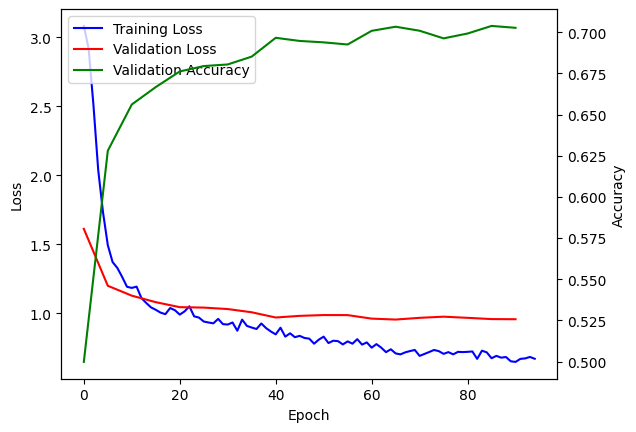
\includegraphics[width=0.8\textwidth]{figures/small_vocab_training_plot.png}
    \caption{CRNN model training history on small vocabualary. We see the training loss and the validation loss and accuracy. The accuracy here is over all chord labels, not ignoring \texttt{X} as in final metric calculations. Training was stopped early at epoch 79. We can see the validation loss flattening out after around epoch 50. However, the model could have continued to be trained as it has not started overfitting yet. This behaviour later contributed to the argument for the removal of early stopping.}\label{fig:crnn_small_vocab_loss}
\end{figure}

Results are shown in Table~\ref{tab:crnn_small_vocab}. For comparison, the table also shows the performance of the same model trained with the large vocabulary, $V=170$ and its predictions mapped back to the smaller vocabualary. A confusion matrix over chord roots of the model trained on $V=25$ is shown in Figure~\ref{fig:crnn_small_vocab_cm}. We see that...


\begin{table}[h]
    \centering
    \begin{tabular}{lcccccc}
        \toprule
        Model & $V$ for training & root & third & class\textsubscript{mean} & class\textsubscript{median} \\  
        \midrule
        \emph{CRNN} & 25 & 0.75 & 0.73 & 0.71 & 0.71 \\
        \emph{CRNN} & 170 & 0.75 & 0.72 & 0.71 & 0.73 \\
        \bottomrule
    \end{tabular}
    \caption{CRNN model results on the small vocabualary with $V=25$. Other metrics are omitted as they are identical for classification with $V=25$.}
    \label{tab:crnn_small_vocab}
\end{table}

While some other works continue to measure performance on the smaller vocabualary~\citep{BTC}, we believe more metrics distract from the main goal of increasing performance across a wider range of chords. Additionally, the inherent ambiguity of whether a chord should be present in the smaller vocabualary will always lead to some chords being misclassified. We therefore only measure performance on the larger vocabualary from now on.

\subsection{Hyperparameter Tuning}

After progressing to the larger vocabualary, we thought it a good time to conduct some hyperparameter tuning. 

\subsubsection{Learning rates}

The first set of hyperparameters experiments was a gridsearch on learning rates and learning rate schedulers as for the \emph{Logistic} model. The learning rates were in the set of \texttt{[0.1, 0.01, 0.001, 0.0001]} and the learning rate schedulers to \texttt{[Cosine, ReduceLROnPlateau, None]}. We remove early stopping in order to check for convergence and overfitting without the possibility of a pre-emptive stop. The best performing model by validation metrics was found to be with \texttt{lr=0.001} and \texttt{Cosine} scheduling. We report a subset of metrics in Table~\ref{tab:crnn_lr}. A sample of training histories are shown in Figure~\ref{fig:crnn_lr}. These figures, alongside Figure~\ref{fig:crnn_small_vocab_loss}, show that the model is not quick to overfit, perhaps due to the random sampling in the training process. Combined with the fact that training is relatively quick and we only save on improved valiation loss, we conclude that early stopping is not necessary. We therefore conduct future experiments without early stopping and with the above learning rate and scheduler.

\subsubsection{Model Hyperparameters}

With this learning rate and learning rate scheduler fixed, we perform a random search on the number of layers in the GRU, the hidden size of the layers in the GRU and the training patch segment length. The search is performed by independently and uniformly randomly sampling 32 points in the sets $\texttt{hidden\_size}\in\{64,65,\ldots,512\}$, $\texttt{num\_layers}\in\{1,2,3\}$ and $\texttt{segment\_length}\in\{10,11,\ldots,60\}$. A sample of the results are shown in Table~\ref{tab:crnn_hparams}. The models were then ranked according to each metric and their ranks for each metric added up. The models were ordered by this total rank. The best model was found to have a hidden size of $201$, a single layer GRU and a segment length of $28$, although the differences between models were relatively small.

\subsection{Model Analysis}
- Transition frame analysis
- Incorrect region analysis
- Worst Songs
\subsection{Long Run SGD}
- Convergence found to be sometimes better with a long run with SGD [XX]
- Results:
\subsection{Hop Length}

- Couldn't test on some of the smaller hop lengths due to Nyquist frequency.
- Instead, tested on 4096, 8192, 16384 and also one smaller on 2896 which is 4096/sqrt(2). 

\section{Weighted Loss}

\section{Pitch Augmentation}
- Two methods:
- On CQT [2019] not good
- Using MUDA on the audio [everyone else], works?

\section{Structured Training}

- Add structured loss and retrain. From literature. Should (?) further improve accuracies on sevenths etc.

\section{Transformer}

- Make own transformer architecture, similar to BTC or HarmonyTransformer, or Curriculum learning. How to train and evaluate?

\section{Using Generative Features}

- As in [MelodyTranscriptionViaGenerativePreTraining], use Jukebox (?) to generate features at frames (? is it possible to do it on the same frames?). Train on these features and evaluate.

\section{Results on Test Set}

- Directly compare CRNN, weighted loss, pitch augmentation, structured, transformer, generative features on the test set.